\documentclass{extbook}[14pt]
\usepackage{multicol, enumerate, enumitem, hyperref, color, soul, setspace, parskip, fancyhdr, amssymb, amsthm, amsmath, latexsym, units, mathtools}
\everymath{\displaystyle}
\usepackage[headsep=0.5cm,headheight=0cm, left=1 in,right= 1 in,top= 1 in,bottom= 1 in]{geometry}
\usepackage{dashrule}  % Package to use the command below to create lines between items
\newcommand{\litem}[1]{\item #1

\rule{\textwidth}{0.4pt}}
\pagestyle{fancy}
\lhead{}
\chead{Answer Key for Progress Quiz 5 Version C}
\rhead{}
\lfoot{8497-6012}
\cfoot{}
\rfoot{Summer C 2021}
\begin{document}
\textbf{This key should allow you to understand why you choose the option you did (beyond just getting a question right or wrong). \href{https://xronos.clas.ufl.edu/mac1105spring2020/courseDescriptionAndMisc/Exams/LearningFromResults}{More instructions on how to use this key can be found here}.}

\textbf{If you have a suggestion to make the keys better, \href{https://forms.gle/CZkbZmPbC9XALEE88}{please fill out the short survey here}.}

\textit{Note: This key is auto-generated and may contain issues and/or errors. The keys are reviewed after each exam to ensure grading is done accurately. If there are issues (like duplicate options), they are noted in the offline gradebook. The keys are a work-in-progress to give students as many resources to improve as possible.}

\rule{\textwidth}{0.4pt}

\begin{enumerate}\litem{
For the graph below, find the value(s) $a$ that makes the statement true: $ \displaystyle \lim_{x \rightarrow a} f(x) = 0$.

\begin{center}
    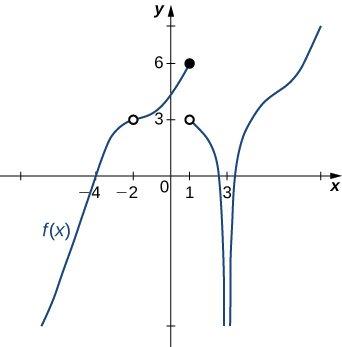
\includegraphics[width=0.5\textwidth]{../Figures/evaluateLimitGraphicallyCopyC.png}
\end{center}


The solution is \( \text{Multiple } a \text{ make the statement true}. \), which is option D.\begin{enumerate}[label=\Alph*.]
\item \( -4 \)


\item \( 0 \)


\item \( 3 \)


\item \( \text{Multiple } a \text{ make the statement true}. \)


\item \( \text{No } a \text{ make the statement true}. \)


\end{enumerate}

\textbf{General Comment:} \textbf{General Comments:} There can be multiple $a$ values that make the statement true! For the limit, draw a horizontal line and determine if an $x$ value makes the limit exist.
}
\litem{
Evaluate the one-sided limit of the function $f(x)$ below, if possible.
\[ \lim_{x \rightarrow 2^-} \frac{-7}{(x-2)^4}+4 \]The solution is \( -\infty \), which is option C.\begin{enumerate}[label=\Alph*.]
\item \( f(2) \)


\item \( \infty \)


\item \( -\infty \)


\item \( \text{The limit does not exist} \)


\item \( \text{None of the above} \)


\end{enumerate}

\textbf{General Comment:} \textbf{General comments:} You should be able to graph the rational function displayed. If not, go back to Module 7 to learn about the general shape of rational functions.
}
\litem{
Evaluate the limit below, if possible.
\[ \lim_{x \rightarrow 9} \frac{\sqrt{7x - 27} - 6}{6x - 54} \]The solution is \( \text{None of the above} \), which is option E.\begin{enumerate}[label=\Alph*.]
\item \( 0.441 \)

You likely tried to use a shortcut to find the limit of a function that only works for when the numerator/denominator are polynomials.
\item \( 0.014 \)

You likely learned L'Hospital's Rule in a previous course, but misapplied it here.
\item \( \infty \)

You likely believed that since the denominator is equal to 0, the limit is infinity.
\item \( 0.083 \)

You likely memorized how to solve the similar homework problem and used the same formula here.
\item \( \text{None of the above} \)

* This is the correct option as the limit is 0.097.
\end{enumerate}

\textbf{General Comment:} \textbf{General comments:} It is difficult to imagine the graph of this function, so you need to test values close to $x = 9$.
}
\litem{
Based on the information below, which of the following statements is always true?

\begin{center}
    \textit{ As $x$ approaches $3$, $f(x)$ approaches $\infty$. }
\end{center}
The solution is \( f(x) \text{ is undefined when } x \text{ is close to or exactly } 3. \), which is option D.\begin{enumerate}[label=\Alph*.]
\item \( f(x) \text{ is close to or exactly } 3 \text{ when } x \text{ is large enough}. \)


\item \( x \text{ is undefined when } f(x) \text{ is close to or exactly } \infty. \)


\item \( f(x) \text{ is close to or exactly } \infty \text{ when } x \text{ is large enough}. \)


\item \( f(x) \text{ is undefined when } x \text{ is close to or exactly } 3. \)


\item \( \text{None of the above are always true.} \)


\end{enumerate}

\textbf{General Comment:} The limit tells you what happens as the $x$-values approach $3$. It says \textbf{absolutely nothing} about what is happening exactly at $f(3)$!
}
\litem{
For the graph below, evaluate the limit: $ \displaystyle \lim_{x \rightarrow -2} f(x)$.

\begin{center}
    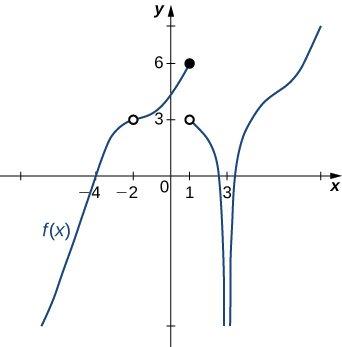
\includegraphics[width=0.5\textwidth]{../Figures/evaluateLimitGraphicallyC.png}
\end{center}


The solution is \( 3 \), which is option C.\begin{enumerate}[label=\Alph*.]
\item \( -\infty \)


\item \( -2 \)


\item \( 3 \)


\item \( \text{The limit does not exist} \)


\item \( \text{None of the above} \)


\end{enumerate}

\textbf{General Comment:} \textbf{General Comments:} Remember that the limit does not exist if the left-hand and right-hand limits do not match.
}
\litem{
Evaluate the limit below, if possible.
\[ \lim_{x \rightarrow 7} \frac{\sqrt{5x - 10} - 5}{3x - 21} \]The solution is \( 0.167 \), which is option D.\begin{enumerate}[label=\Alph*.]
\item \( 0.100 \)

You likely memorized how to solve the similar homework problem and used the same formula here.
\item \( 0.745 \)

You likely tried to use a shortcut to find the limit of a function that only works for when the numerator/denominator are polynomials.
\item \( \infty \)

You likely believed that since the denominator is equal to 0, the limit is infinity.
\item \( 0.167 \)

* This is the correct option.
\item \( \text{None of the above} \)

If you got a limit that does not match any of the above, please contact the coordinator.
\end{enumerate}

\textbf{General Comment:} \textbf{General comments:} It is difficult to imagine the graph of this function, so you need to test values close to $x = 7$.
}
\litem{
Evaluate the one-sided limit of the function $f(x)$ below, if possible.
\[ \lim_{x \rightarrow 3^+} \frac{-1}{(x-3)^4}+8 \]The solution is \( -\infty \), which is option A.\begin{enumerate}[label=\Alph*.]
\item \( -\infty \)


\item \( \infty \)


\item \( f(3) \)


\item \( \text{The limit does not exist} \)


\item \( \text{None of the above} \)


\end{enumerate}

\textbf{General Comment:} \textbf{General comments:} You should be able to graph the rational function displayed. If not, go back to Module 7 to learn about the general shape of rational functions.
}
\litem{
To estimate the one-sided limit of the function below as $x$ approaches 8 from the left, which of the following sets of numbers should you use?
\[ \frac{\frac{8}{x} - 1}{x - 8} \]The solution is \( \{ 7.9000, 7.9900, 7.9990, 7.9999 \} \), which is option E.\begin{enumerate}[label=\Alph*.]
\item \( \{ 8.0000, 8.1000, 8.0100, 8.0010 \} \)

If we get $\frac{0}{0}$ or $\frac{\infty}{\infty}$, the value 8 doesn't help us estimate the limit.
\item \( \{ 7.9000, 7.9900, 8.0100, 8.1000 \} \)

These values would estimate the limit at the point and not a one-sided limit.
\item \( \{ 8.0000, 7.9000, 7.9900, 7.9990 \} \)

If we get $\frac{0}{0}$ or $\frac{\infty}{\infty}$, the value 8 doesn't help us estimate the limit.
\item \( \{ 8.1000, 8.0100, 8.0010, 8.0001 \} \)

These values would estimate the limit of 8 on the right.
\item \( \{ 7.9000, 7.9900, 7.9990, 7.9999 \} \)

This is correct!
\end{enumerate}

\textbf{General Comment:} \textbf{General Comments:} To evaluate a one-sided limit, we want to put numbers close to the limit. We can't use the limit value itself if it results in $\frac{0}{0}$ or $\frac{\infty}{\infty}$
}
\litem{
To estimate the one-sided limit of the function below as $x$ approaches 9 from the left, which of the following sets of numbers should you use?
\[ \frac{\frac{9}{x} - 1}{x - 9} \]The solution is \( \{ 8.9000, 8.9900, 8.9990, 8.9999 \} \), which is option B.\begin{enumerate}[label=\Alph*.]
\item \( \{ 9.0000, 8.9000, 8.9900, 8.9990 \} \)

If we get $\frac{0}{0}$ or $\frac{\infty}{\infty}$, the value 9 doesn't help us estimate the limit.
\item \( \{ 8.9000, 8.9900, 8.9990, 8.9999 \} \)

This is correct!
\item \( \{ 9.1000, 9.0100, 9.0010, 9.0001 \} \)

These values would estimate the limit of 9 on the right.
\item \( \{ 8.9000, 8.9900, 9.0100, 9.1000 \} \)

These values would estimate the limit at the point and not a one-sided limit.
\item \( \{ 9.0000, 9.1000, 9.0100, 9.0010 \} \)

If we get $\frac{0}{0}$ or $\frac{\infty}{\infty}$, the value 9 doesn't help us estimate the limit.
\end{enumerate}

\textbf{General Comment:} \textbf{General Comments:} To evaluate a one-sided limit, we want to put numbers close to the limit. We can't use the limit value itself if it results in $\frac{0}{0}$ or $\frac{\infty}{\infty}$
}
\litem{
Based on the information below, which of the following statements is always true?

\begin{center}
    \textit{ As $x$ approaches $8$, $f(x)$ approaches $12.177$. }
\end{center}
The solution is \( \text{None of the above are always true.} \), which is option E.\begin{enumerate}[label=\Alph*.]
\item \( f(8) \text{ is close to or exactly } 12 \)


\item \( f(8) = 12 \)


\item \( f(12) \text{ is close to or exactly } 8 \)


\item \( f(12) = 8 \)


\item \( \text{None of the above are always true.} \)


\end{enumerate}

\textbf{General Comment:} The limit tells you what happens as the $x$-values approach $8$. It says \textbf{absolutely nothing} about what is happening exactly at $f(8)$!
}
\end{enumerate}

\end{document}